%!TEX root = paper.tex


\section{Fault Tolerance via Asynchronous Snapshots}
\label{sec:snapshots}
Before jumping to the higher layers of the system, we detail how the common fabric (Flink’s runtime) guarantees consistent results in the case of failures. Since Flink data streams are replayable, discarding partial results and re-producing the lost partitions of the resulting streams (which possibly may trigger partial re-computation down to the sources in the case of non-buffered streams) is enough to guarantee fault tolerance when the computation is finite \cite{DBLP:conf/hotcloud/ZahariaCFSS10}. This is the mechanism used for Flink DataSet (batch) API programs.

In stream processing (Flink’s DataStream API), the computation is possibly infinite, which makes the above approach not practical, as possibly months of computation will need to be replayed. To bound recovery time, Flink takes a snapshot of the state of operators, including the current position of the input streams at regular intervals.

The core challenge lies in taking a consistent snapshot of all parallel operators without stopping the topology. In essence, the snapshot of all operators should refer to the same logical time in the computation. The mechanism used in Flink is called Asynchronous Barrier Snapshotting, or ABS \cite{carbone2015lightweight}. Barriers are messages injected into the input streams that correspond to a logical time, and logically separate the stream to the part whose effects will be included in the current snapshot, and the part that will be snapshotted later.

\begin{figure}[ht]
	\centering  	
  	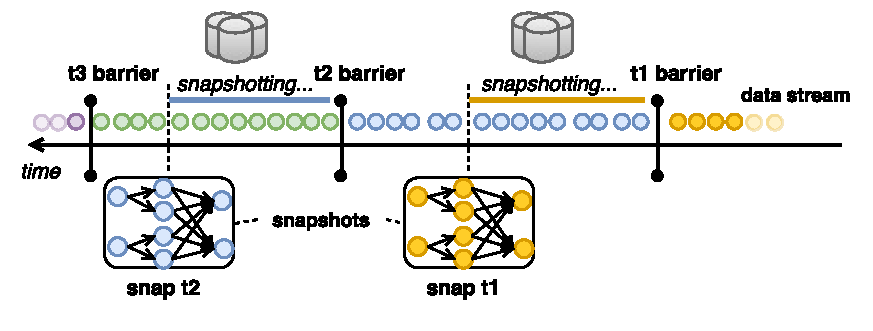
\includegraphics[width=.75\textwidth]{figs/snaps.pdf}
  	\vspace{-4mm}
	\caption{Asynchronous Barrier Snapshotting.}
	\vspace{-2mm}
	\label{fig:FlinkStack}
\end{figure}

An operator receives barriers from upstream and first performs an alignment phase, making sure that the barriers from all inputs have been received. Then, the operator writes its state (e.g., contents of a sliding window, or custom data structures) to durable storage (the storage backend can be an external system, e.g., HDFS). Once the state has been backed up, the operator forwards the barrier downstream. ABS bears resemblances to the seminal Chandy-Lamport algorithm for asynchronous distributed snapshots \cite{chandy1985distributed}. However, because of the DAG structure of a Flink program and the alignment phase, ABS does not need to checkpoint in-flight records, guaranteeing that the data that needs to be written to reliable storage is kept to the theoretical minimum (i.e., only the current state of the operators).


Recovery from failures reverts the operator state to the most recently snapshotted one, and restarts the input streams from the latest barrier. This guarantees that the replayed work is limited to the processing between two checkpoints. We note that recovery need not start from the sources if intermediate streams have been partially buffered.

\vspace{2mm}
\noindent ABS provides several benefits: 

\begin{itemize}
\item It guarantees exactly-once state updates without ever pausing the computation (e.g., as compared to discretized streams \cite{DBLP:conf/hotcloud/ZahariaCFSS10} which is essentially a synchronous implementation of snapshotting).
\item It is completely decoupled other forms of control messages, e.g., by events that trigger the computation of windows, thus not restricting the windowing mechanism to multiples of the checkpoint interval (again compare with \cite{DBLP:conf/hotcloud/ZahariaCFSS10})
\item It is completely decoupled from the mechanism used for reliable storage, allowing state to be backed up to file systems, databases, etc, depending on the larger environment in which Flink is used.
\end{itemize}


